\documentclass[11pt,a4paper]{jsarticle}
%
\usepackage{amsmath,amssymb}
\usepackage{bm}
\usepackage[dvipdfmx]{graphicx}
\usepackage{ascmac}
%
\setlength{\textwidth}{\fullwidth}
\setlength{\textheight}{40\baselineskip}
\addtolength{\textheight}{\topskip}
\setlength{\voffset}{-0.2in}
\setlength{\topmargin}{0pt}
\setlength{\headheight}{0pt}
\setlength{\headsep}{0pt}
%
\newcommand{\divergence}{\mathrm{div}\,}  %ダイバージェンス
\newcommand{\grad}{\mathrm{grad}\,}  %グラディエント
\newcommand{\rot}{\mathrm{rot}\,}  %ローテーション
%



\title{単語クイズを自動生成して楽しみながら覚えるWebアプリケーションの考案}
\author{k22120 牧野遥斗}
\date{\today}


\begin{document}

\begin{titlepage}
    \begin{center}

        \ \vspace{19mm}

        \LARGE\baselineskip=13mm
        Webプログラミング基礎\\[1mm]
        {\Huge\baselineskip=13mm
        \textbf{単語クイズを自動生成して楽しみながら覚えるWebアプリケーションの考案} \\
        }

        \vspace{80mm}

        \kanjiskip=9pt plus 1pt minus1pt
        \today \\
        K22120\hspace{1zw}牧野遥斗 \\
    \end{center}
\end{titlepage}

% \maketitle
\section{目的}
このアプリケーションは、日々の授業や資格取得など数多くある単語を楽しんで覚えるために使うWebアプリケーションである。

我々は外国語の勉強をする時には数多くの単語を覚える必要がある。
英語だったり、フランス語だったり、日本語だったり、その他の言語でも同じだ。しかし、単語を覚えるのはとても大変である。
単語を覚えるには、単語帳を使うのが一般的だ。しかし、単語帳を使うと、単語を覚えるのに時間がかかる。また、単語帳を使うと、単語を覚えるのに面白みがない。
そこで、我々は、単語を覚えるのに面白みを持たせることで、単語を覚えるのに時間を短縮することを目的としている。

\section{機能}
このアプリケーションは、単語クイズを自動生成して楽しみながら覚えることができる。
そのため、単語を登録する編集画面と、単語をクイズするクイズ画面がある。

\begin{figure}[htbp]
    \begin{minipage}{0.5\hsize}
        \begin{center}
            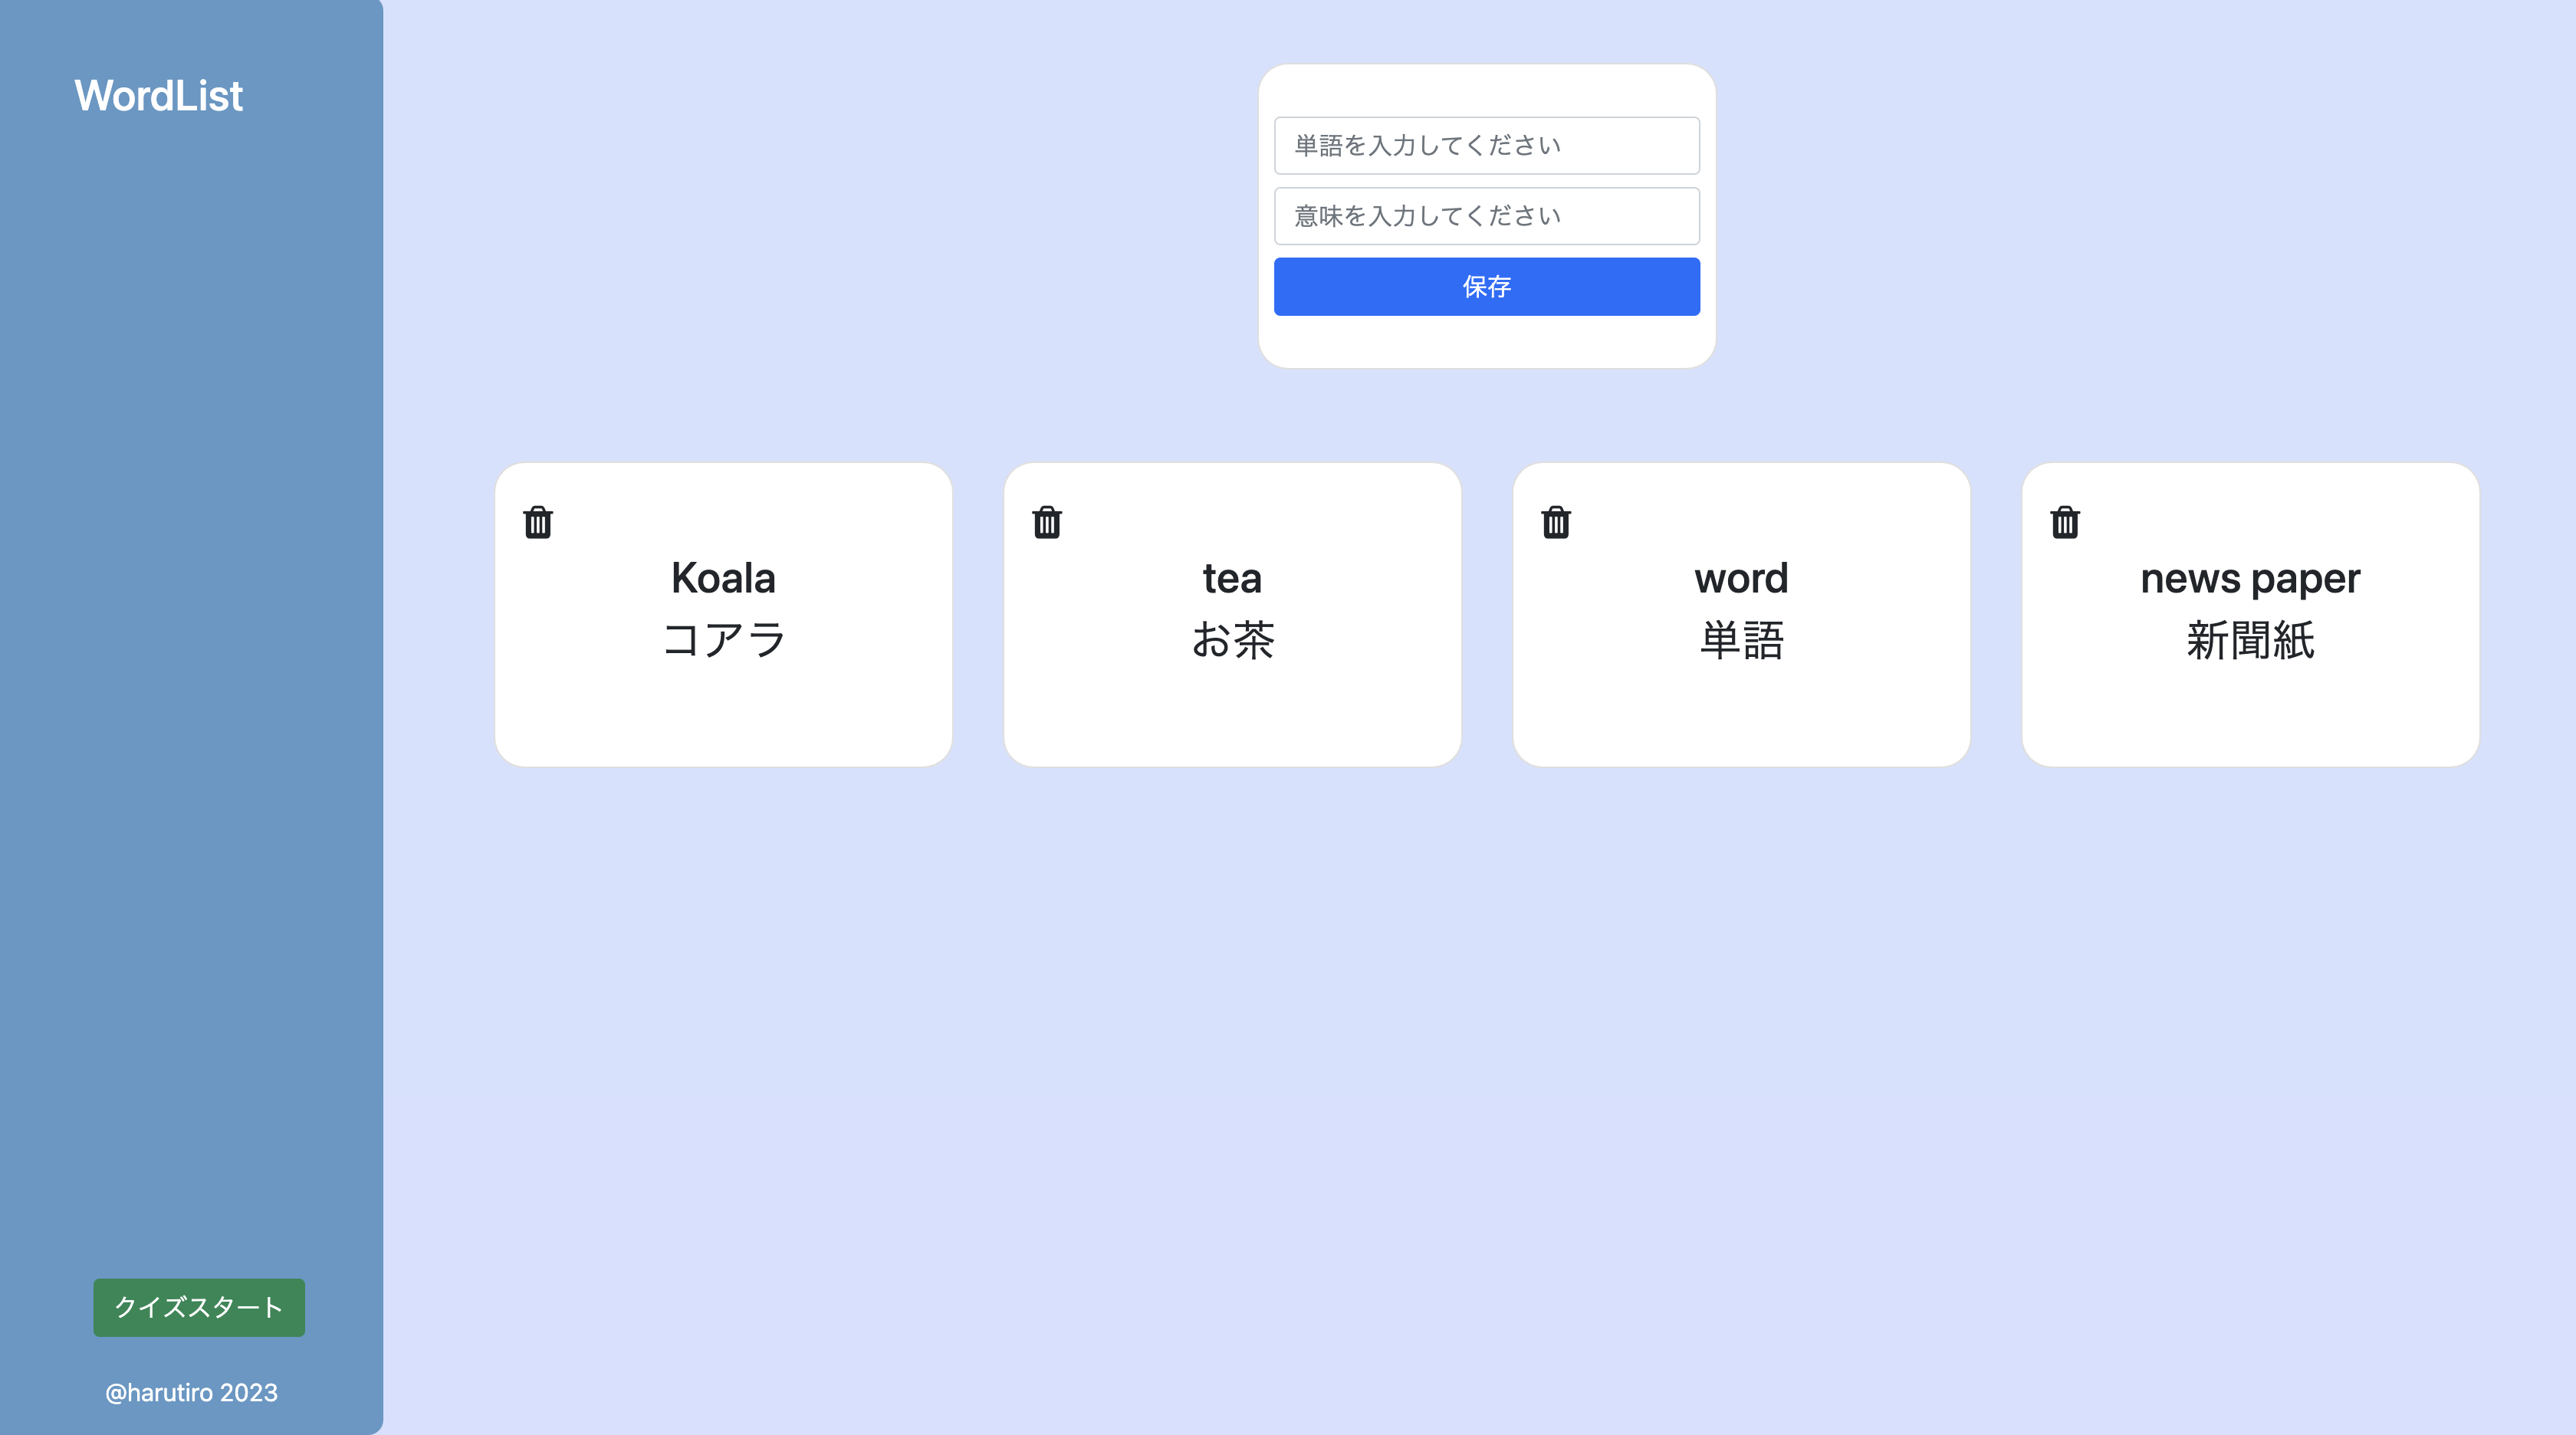
\includegraphics[width=70mm]{./img/edit_screen.png}
        \end{center}
        \caption{編集画面}
    \end{minipage}
    \begin{minipage}{0.5\hsize}
        \begin{center}
            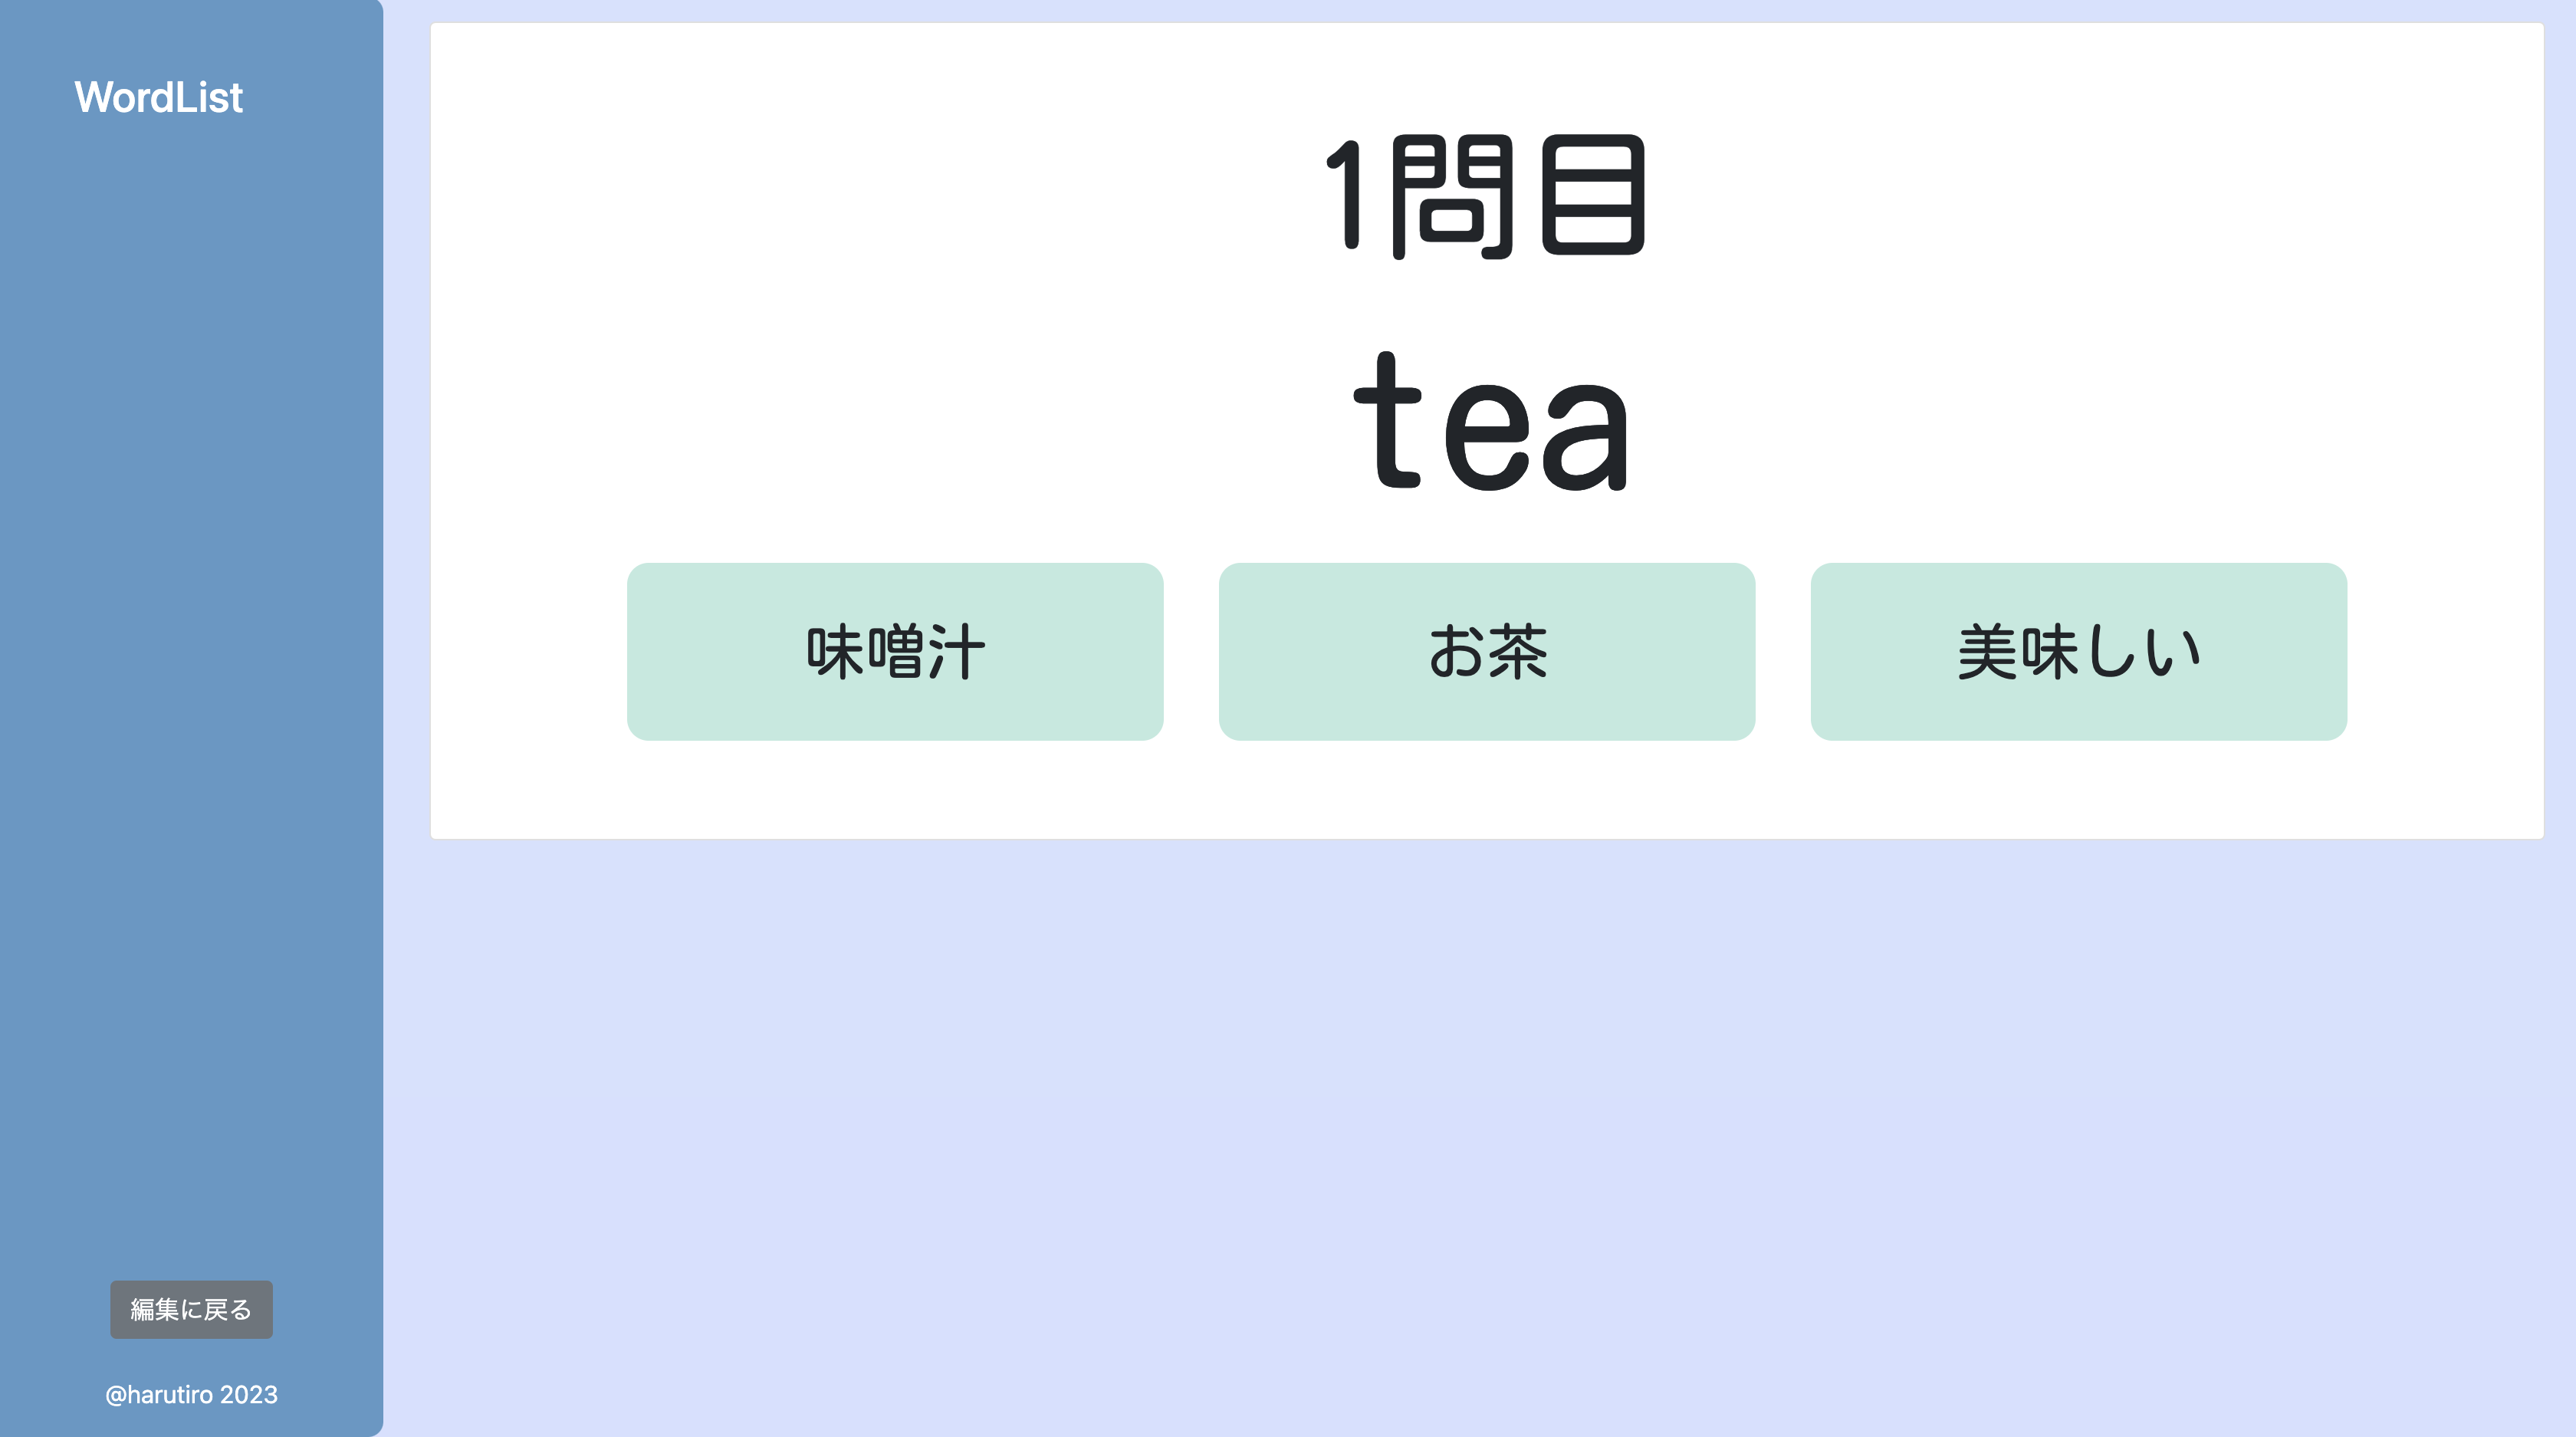
\includegraphics[width=70mm]{./img/quiz_screen.png}
        \end{center}
        \caption{クイズ画面}
    \end{minipage}
\end{figure}

\subsection{編集画面}
編集画面では、単語とその意味を登録することができる。
単語とその意味を登録すると、クイズの自動生成ができるかどうかを判定する。
クイズの自動生成ができる単語は、今回APIで使用したWordVecの単語ベクトルに含まれている単語である。
Word2Vecの詳しい説明は、節\ref{sec:Word2Vec}に記載する。
クイズの自動生成ができない単語のエラー画面は図\ref{fig:quiz_error}に示す。
エラーを表示することにより、クイズの自動生成ができない単語を登録することを防ぎ、クイズの自動生成ができる単語のみを登録することができる。

%画像を出力する
\begin{figure}[htbp]
    \begin{center}
        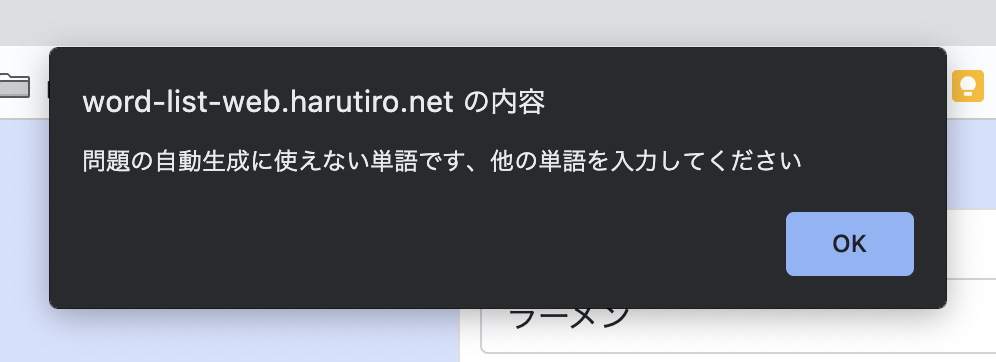
\includegraphics[width=70mm]{./img/error_popup.png}
    \end{center}
    \caption{クイズの自動生成ができない単語のエラー画面}
    \label{fig:quiz_error}
\end{figure}

覚えたい単語を登録しおえたら、クイズ画面に移動することができる。
左下の緑のボタン「クイズスタート」を押し、クイズ画面に移動する。

\subsection{クイズ画面}
クイズ画面では、単語クイズを自動生成して楽しみながら覚えることができる。
クイズは3択クイズで、単語の意味を選択することができる。
クイズの自動生成は、Word2Vecの単語ベクトルを用いて行う。
正解の単語の意味に近い単語を50件取得し、その単語の中から二種類選択肢として表示する。

最後のクイズが終わった後に、クイズを終了したアナウンスを表示する。


\begin{figure}[htbp]
    \begin{center}
        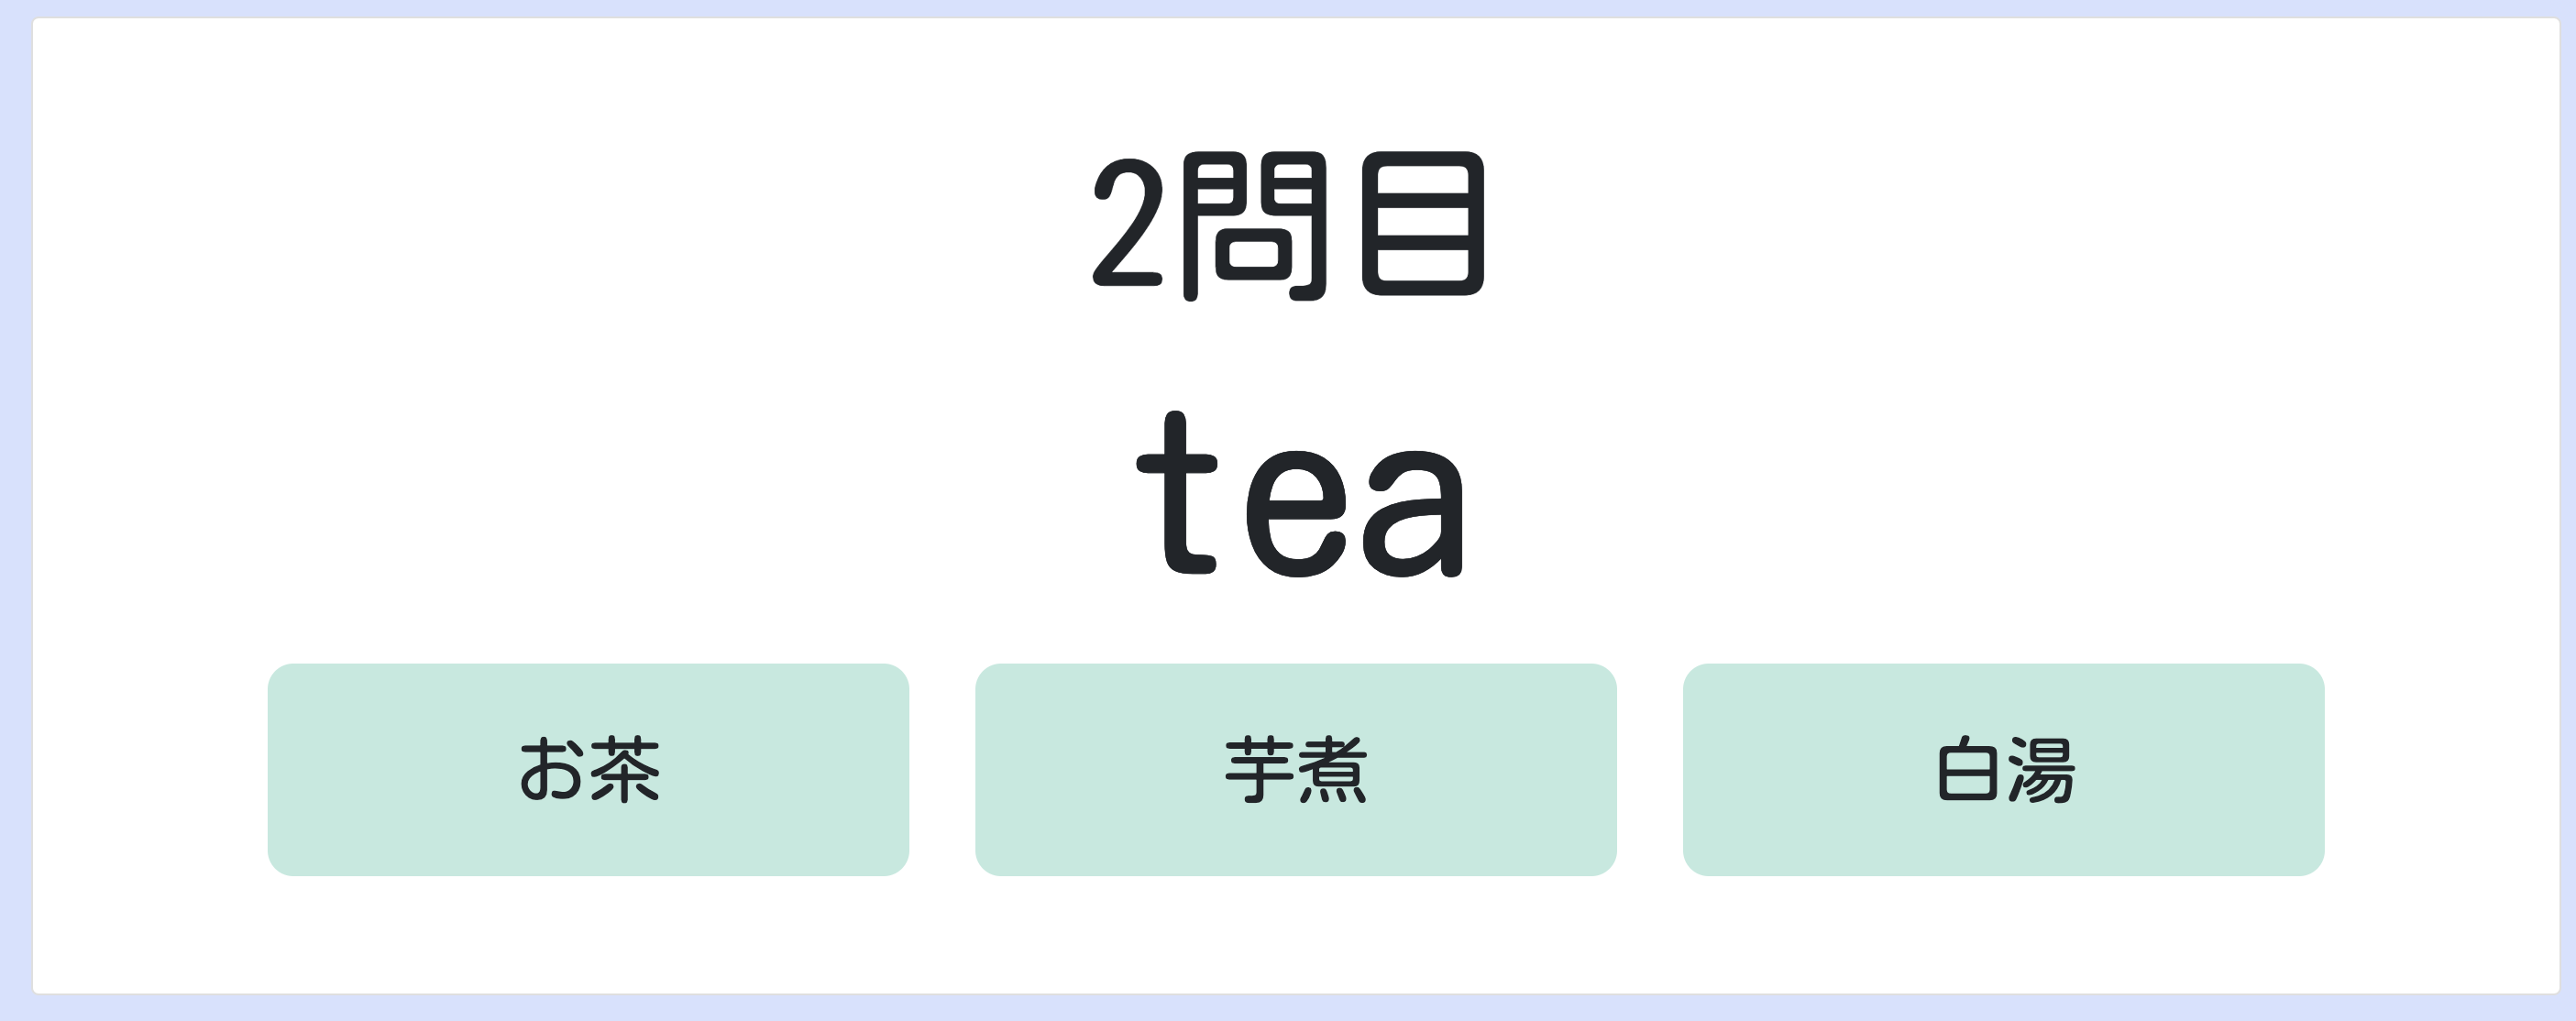
\includegraphics[width=70mm]{./img/question.png}
    \end{center}
    \caption{クイズの選択画面}
\end{figure}


\begin{figure}[htbp]
    \begin{center}
        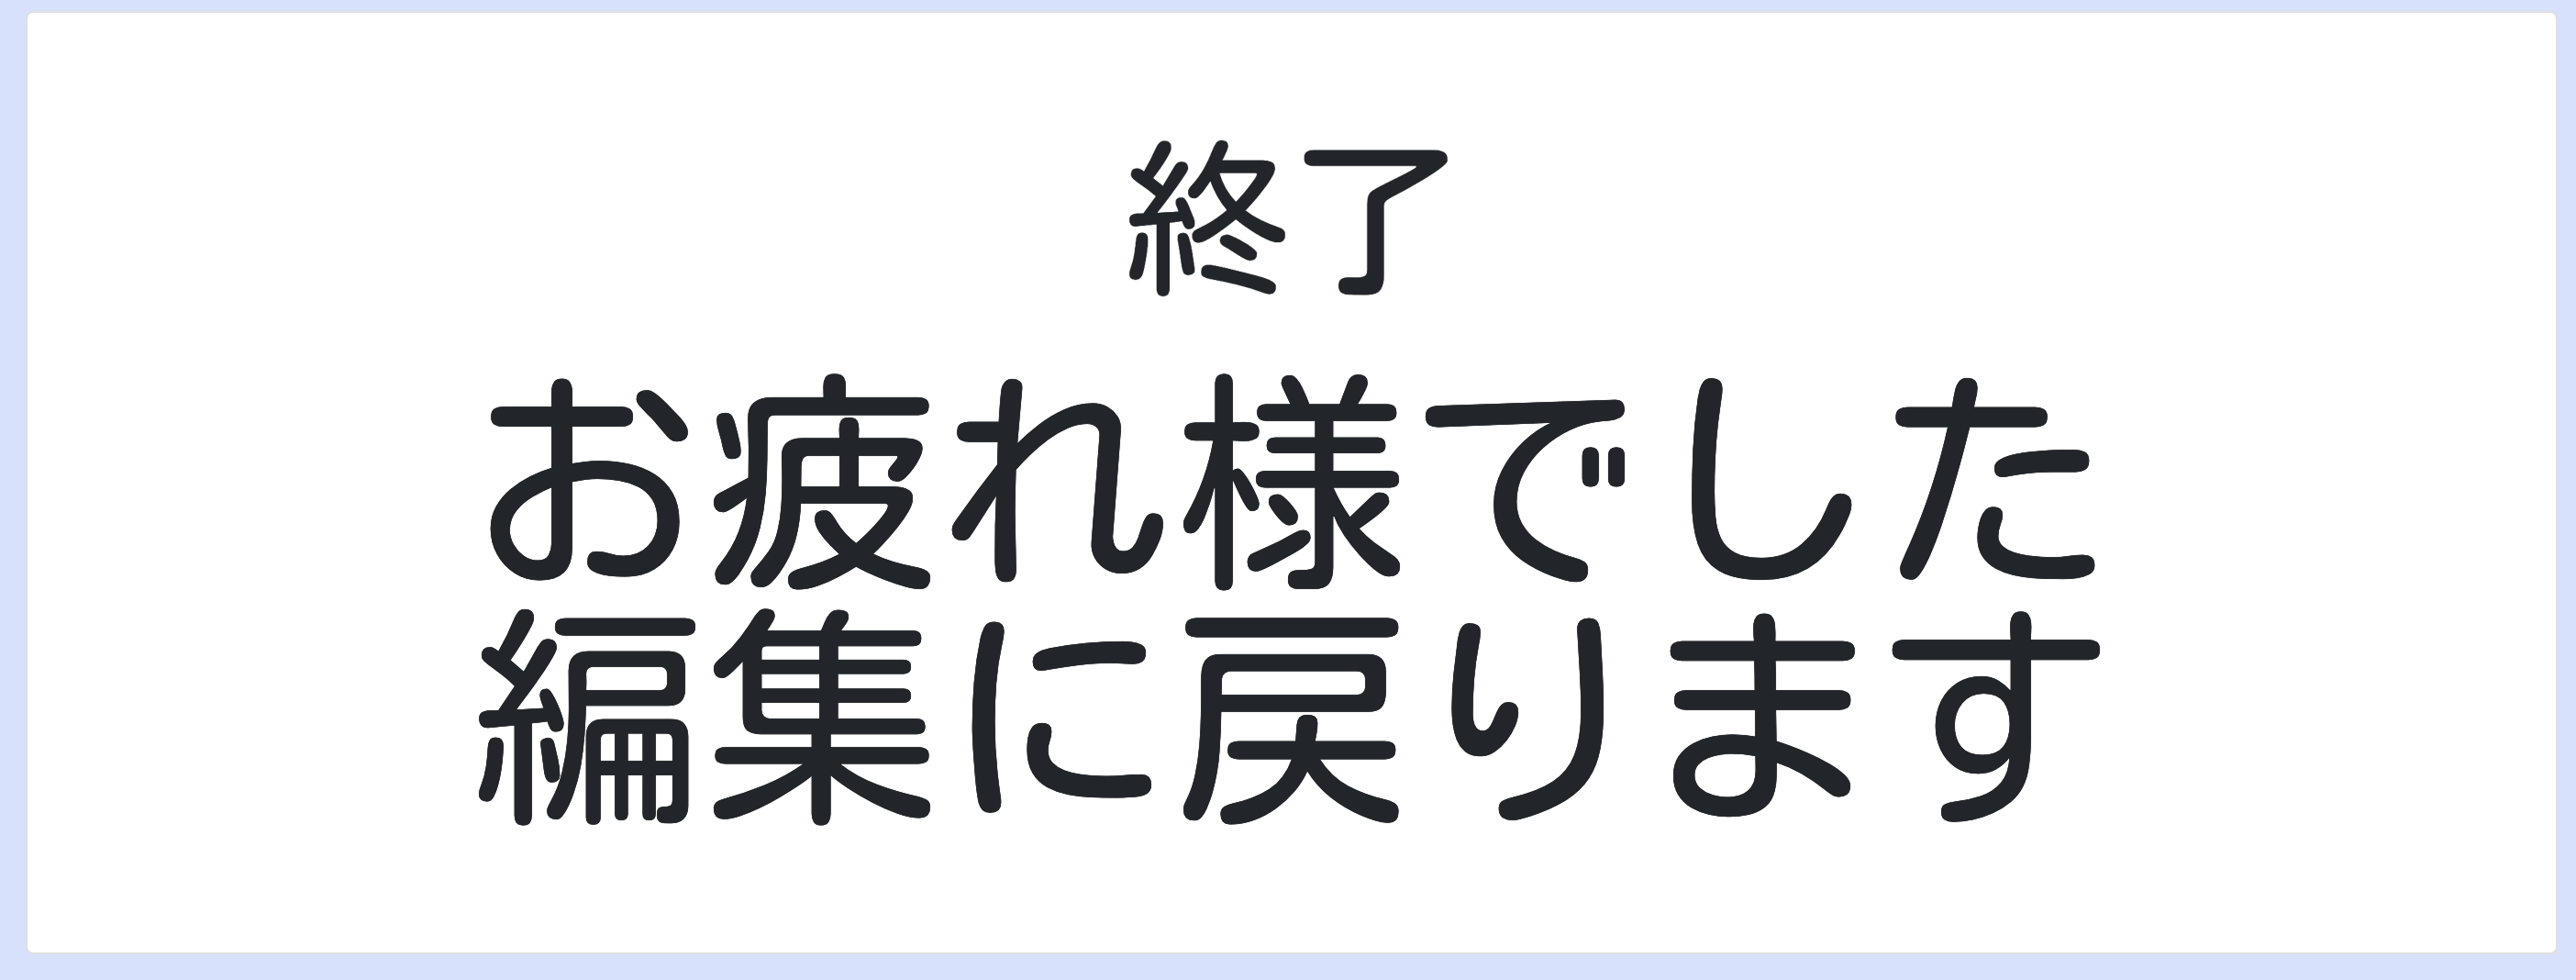
\includegraphics[width=70mm]{./img/question_end.png}
    \end{center}
    \caption{クイズの終了画面}
\end{figure}



\section{目的}

単語を覚えるのに面白みを持たせることで、単語を覚えるのに時間を短縮することを目的としている。
単語を覚えるのに面白みを持たせるために、単語をクイズ形式で覚えることができる。
クイズを作成する時に、自分ですべての問題を作るというのは大変である。
そこで、単語の意味を入力するだけで、クイズを自動生成することができるようにした。
Word2Vecを用いることで、単語の意味を入力するだけで、単語の意味に近い単語を取得することができ、簡単にクイズを作成することができる。

機能面は、単語を登録し、クイズをするという中核をなす部分は完成している。



\subsection{改善点}
今後の改善点として、以下のようなものがある。
様々な単語を登録することで、様々なジャンルの単語が乱立してしまい覚えたい単語以外の単語もクイズに出てきてしまう問題点がある。
この問題点を解決するために、単語を登録する際に、単語のジャンルを登録することができるようにする。
単語のジャンルを登録することで、単語のジャンルを指定してクイズを出題することができる。

次に、Word2Vecの単語ベクトルを用いてクイズを自動生成しているため、単語ベクトルにない言葉はクイズに出題できない。
今回はWikipediaの記事をサンプルとして使用しているため、日本語以外の言語は単語ベクトルにあまり含まれていない。
この問題点を解決するために、英語版のWikipediaをサンプルとして使用することで、単語ベクトルに含まれていない単語もクイズに出題することができる。
また、中国語やフランス語にも対応させるため、世界各国のサンプルデータを取得することで、単語ベクトルに含まれていない単語もクイズに出題することができる。

\section{付録}

\subsection{Word2Vec}\label{sec:Word2Vec}

\subsection{API通信部分}







\end{document}
